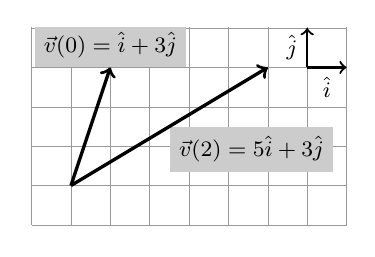
\begin{tikzpicture}[scale=0.5, help lines/.style={black!40,very thin}]
	\clip (-1.1,-1.1) rectangle (7.01,4.01);

	% Grid
	\draw[help lines] (-1,-1) grid +(8,9);

	% \vec v(0)
	\draw (1,3) node[anchor=south, fill=black!20!white] {\footnotesize $\vec v(0) = \hat i + 3\hat j$};
	\draw[very thick] [->] (0,0) -- (1,3);

	% \vec v(2)
	\draw (2.5,1.5) node[anchor=north west, fill=black!20!white] {\footnotesize $\vec v(2) = 5\hat i + 3\hat j$};
	\draw[very thick] [->] (0,0) -- (5,3);

	% \hat i
	\draw (6.5,3) node[anchor=north] {\footnotesize $\hat i$};
	\draw[thick] [->] (6,3) -- ++(1,0);

	% \hat j
	\draw (6,3.5) node[anchor=east] {\footnotesize $\hat j$};
	\draw[thick] [->] (6,3) -- ++(0,1);
\end{tikzpicture}
